\documentclass[10pt,english]{beamer}
\usepackage{lmodern}
\usepackage[T1]{fontenc}
\usepackage[utf8]{inputenc}
\setcounter{tocdepth}{1}
\usepackage{amsbsy}
\usepackage{amstext}
\usepackage{amssymb}
\usepackage[authoryear]{natbib}

\makeatletter
%%%%%%%%%%%%%%%%%%%%%%%%%%%%%% Textclass specific LaTeX commands.
% this default might be overridden by plain title style
\newcommand\makebeamertitle{\frame{\maketitle}}%
% (ERT) argument for the TOC
\AtBeginDocument{%
  \let\origtableofcontents=\tableofcontents
  \def\tableofcontents{\@ifnextchar[{\origtableofcontents}{\gobbletableofcontents}}
  \def\gobbletableofcontents#1{\origtableofcontents}
}

%%%%%%%%%%%%%%%%%%%%%%%%%%%%%% User specified LaTeX commands.



\usepackage{tikz}
\usetikzlibrary{positioning}
\usepackage{appendixnumberbeamer}

\usepackage{graphicx}
\usepackage{subfig}

\usetheme[progressbar=frametitle,block=fill,subsectionpage=progressbar]{metropolis}

% margin
\setbeamersize{text margin right=1.5cm}

% colors
%\colorlet{DarkRed}{red!70!black}
\definecolor{DarkRed}{rgb}{0.7,0,0}

\setbeamercolor{normal text}{fg=black}
\setbeamercolor{alerted text}{fg=DarkRed}
\setbeamercolor{progress bar}{fg=DarkRed}
\setbeamercolor{button}{bg=DarkRed}

% width of seperators
\makeatletter
\setlength{\metropolis@titleseparator@linewidth}{1pt}
\setlength{\metropolis@progressonsectionpage@linewidth}{1pt}
\setlength{\metropolis@progressinheadfoot@linewidth}{1pt}
\makeatother

% new alert block
\newlength\origleftmargini
\setlength\origleftmargini\leftmargini
\setbeamertemplate{itemize/enumerate body begin}{\setlength{\leftmargini}{4mm}}
\let\oldalertblock\alertblock
\let\oldendalertblock\endalertblock
\def\alertblock{\begingroup \setbeamertemplate{itemize/enumerate body begin}{\setlength{\leftmargini}{\origleftmargini}} \oldalertblock}
\def\endalertblock{\oldendalertblock \endgroup}
\setbeamertemplate{mini frame}{}
\setbeamertemplate{mini frame in current section}{}
\setbeamertemplate{mini frame in current subsection}{}
\setbeamercolor{section in head/foot}{fg=normal text.bg, bg=structure.fg}
\setbeamercolor{subsection in head/foot}{fg=normal text.bg, bg=structure.fg}

% footer
\makeatletter
\setbeamertemplate{footline}{%
    \begin{beamercolorbox}[colsep=1.5pt]{upper separation line head}
    \end{beamercolorbox}
    \begin{beamercolorbox}{section in head/foot}
      \vskip1pt\insertsectionnavigationhorizontal{\paperwidth}{}{\hskip0pt plus1filll \insertframenumber{} / \inserttotalframenumber \hskip2pt}\vskip3pt% 
    \end{beamercolorbox}%
    \begin{beamercolorbox}[colsep=1.5pt]{lower separation line head}
    \end{beamercolorbox}
}
\makeatother

% toc
\setbeamertemplate{section in toc}{\hspace*{1em}\inserttocsectionnumber.~\inserttocsection\par}
\setbeamertemplate{subsection in toc}{\hspace*{2em}\inserttocsectionnumber.\inserttocsubsectionnumber.~\inserttocsubsection\par}



% code
\usepackage{xcolor}
\usepackage{listings}

\definecolor{codegray}{rgb}{0.5,0.5,0.5}
\definecolor{background}{HTML}{F5F5F5}
\definecolor{keyword}{HTML}{4B69C6}
\definecolor{string}{HTML}{448C27}
\definecolor{comment}{HTML}{448C27}

\usepackage{inconsolata}
\lstdefinestyle{mystyle}{
    commentstyle=\color{comment},
    keywordstyle=\color{keyword},
    stringstyle=\color{string},
    basicstyle=\ttfamily,
    breakatwhitespace=false,         
    breaklines=true,                 
    captionpos=b,                    
    keepspaces=true,                                    
    numbersep=5pt,                  
    showspaces=false,                
    showstringspaces=false,
    showtabs=false,
    tabsize=4,
	showlines=true
}

\lstset{style=mystyle}
% Added by lyx2lyx
\setlength{\parskip}{\smallskipamount}
\setlength{\parindent}{0pt}

\makeatother

\newcommand{\ikcdag}[2]{%
\begin{center}
\begin{tikzpicture}[blk/.style={draw,rounded corners=3pt,minimum width=21mm,minimum height=11mm,align=center,font=\small},lab/.style={font=\small,inner sep=2pt},ext/.style={font=\small,align=center,text=DarkRed},arr/.style={->,>=stealth,thick},scale=0.82,every node/.append style={transform shape}]
\node[ext] (sh) at (0,0) {Shock\\$\boldsymbol{r}$};
\node[blk] (go) at (2.6,0) {Government};
\node[blk,fill=DarkRed!20,draw=DarkRed,very thick] (hh) at (5.5,0) {#1\\#2};
\node[blk] (mc) at (8.4,0) {Goods market\\$\boldsymbol{Y}=\boldsymbol{C}+\boldsymbol{G}$};
\node[ext] (tg) at (10.9,0) {Target:\\goods};
\node[ext] (unk) at (6.95,1.75) {Unknown $\boldsymbol{Y}$};
\draw[arr] (sh)--(go);
\draw[arr] (go)--node[lab,above]{$\boldsymbol{T}$}(hh);
\draw[arr] (hh)--node[lab,above]{$\boldsymbol{C}$}(mc);
\draw[arr] (mc)--(tg);
\draw[arr] (unk)--(hh);
\draw[arr] (unk)--(mc);
\draw[arr] (sh.south)--(0,-1.5)--node[lab,below]{$\boldsymbol{r}$}(5.5,-1.5)--(hh.south);
\end{tikzpicture}
\end{center}}
\newcommand{\blockdag}[2]{%
\begin{center}
\begin{tikzpicture}[blk/.style={draw,rounded corners=3pt,minimum height=11mm,align=center,font=\small},lab/.style={font=\small,inner sep=2pt},ext/.style={font=\small,align=center,text=DarkRed},arr/.style={->,>=stealth,thick},scale=0.82,every node/.append style={transform shape}]
\node[ext] (unk) at (-0.2,0) {Unknowns\\$\boldsymbol{\pi}^{w},\boldsymbol{L}$};
\node[blk,dashed,inner sep=5pt] (ma) at (3.2,0) {\begin{tabular}{ll}Firms & $\boldsymbol{Y},\boldsymbol{\pi},\boldsymbol{d}$\\Central bank & $\boldsymbol{r}$\\Government & $\boldsymbol{\tau},\boldsymbol{T}$\\Mutual fund & $\boldsymbol{r}^{p}$\end{tabular}};
\node[blk,fill=DarkRed!20,draw=DarkRed,very thick] (hh) at (7.3,0) {#1\\#2};
\node[blk] (tg) at (10.9,0) {Goods market\\W-NKPC};
\node[ext] (sh) at (3.2,2.05) {Shocks $\boldsymbol{G},\boldsymbol{B},\boldsymbol{\epsilon}^{i}$};
\node[ext] (ok) at (10.9,-1.95) {Targets};
\draw[arr] (unk)--(ma);
\draw[arr] (sh)--(ma);
\draw[arr] (ma)--node[lab,above]{$\boldsymbol{Z},\boldsymbol{r}^{p}$}(hh);
\draw[arr] (hh)--node[lab,above]{$\boldsymbol{C}$}(tg);
\draw[arr] (tg)--(ok);
\draw[arr] (sh)-|node[lab,pos=0.25,above]{$\boldsymbol{G}$}(tg);
\draw[arr] (ma.south) |- node[lab,pos=0.75,below]{$\boldsymbol{Y},\boldsymbol{\pi}^{w},\boldsymbol{L},\boldsymbol{\tau}$} (9.9,-1.3)--(9.9,-0.56);
\end{tikzpicture}
\end{center}}

\usepackage{babel}
\begin{document}
\title{11. Monetary Policy in HANK, part 1\vspace{-2mm}}
\subtitle{Adv. Macro: Heterogeneous Agent Models}
\author{Raphaël Huleux}
\date{2026}

{
\setbeamertemplate{footline}{}
\begin{frame}

\maketitle

\end{frame}
}

\addtocounter{framenumber}{-1}

\section{Introduction}

\begin{frame}{Where we are}
\begin{itemize}
\item <+->\textbf{Fiscal lectures:} same macro blocks, three household blocks, one object $\boldsymbol{M}$
\item <+->With real bonds and a real rate rule, fiscal policy works through $\boldsymbol{M}$:
\[
d\boldsymbol{Y}=d\boldsymbol{G}+\boldsymbol{M}\left(d\boldsymbol{Y}-d\boldsymbol{T}\right)
\]
\item <+->Heterogeneity changes the multiplier, because it changes $\boldsymbol{M}$
\item <+->Monetary policy starts from another object: the response of consumption to the interest rate, $\boldsymbol{M}^{r}$
\end{itemize}
\end{frame}
%
\begin{frame}{Introduction}
\begin{itemize}
\item <+->\textbf{Question:} does heterogeneity change how much monetary policy moves output, and how it does it?
\item <+->\textbf{First session:}
\begin{enumerate}
\item The monetary IKC, and why it needs nominal rigidities
\item RANK and HANK: direct and indirect effects
\item Werning's equivalence result
\item The full model: capital gains, nominal bonds, unequal incidence
\item Forward guidance: does HANK solve the puzzle?
\end{enumerate}
\item <+->\textbf{Second session:} redistribution (Auclert, 2019), expectations and investment (Auclert et al, 2025)
\item <+->\textbf{Literature:}
\begin{itemize}
\item Kaplan, Moll and Violante (2018), >>Monetary Policy According to HANK<<
\item Werning (2015), >>Incomplete Markets and Aggregate Demand<<
\item McKay, Nakamura and Steinsson (2016), >>The Power of Forward Guidance Revisited<<
\end{itemize}
\end{itemize}
\end{frame}
%

\section{NK framework}

\begin{frame}{Reminder: the NK model}
\begin{itemize}
\item <+->Same model as in the fiscal lectures:
\begin{itemize}
\item \textbf{Households:} choose consumption and saving, work as much as the union decides
\item \textbf{Firms:} produce with labor, set prices at a markup, pay dividends
\item \textbf{Unions:} set wages, face a cost of changing wages
\item \textbf{Mutual fund:} collects savings, holds stocks and government bonds
\item \textbf{Government:} sets spending and debt, taxes adjust
\item \textbf{Central bank:} sets the nominal interest rate
\end{itemize}
\item <+->\textbf{One change:} the shock now hits the central bank
\[
i_{t}=i_{ss}+\phi\pi_{t}+\epsilon_{t}^{i},\quad\epsilon_{t}^{i}=\rho_{i}\epsilon_{t-1}^{i}+\eta_{t}^{i}
\]
\end{itemize}
\end{frame}
%
\begin{frame}{Block representation}
\blockdag{Households}{$C^{hh}(\boldsymbol{Z},\boldsymbol{r}^{p})$}
\begin{itemize}
\item <+->\textbf{Read it left to right:} guess $\boldsymbol{\pi}^{w},\boldsymbol{L}$, compute the aggregate blocks, get consumption, check the two targets
\item <+->The red box is left open: RANK and HANK fill it in, nothing else changes
\end{itemize}
\end{frame}
%
\begin{frame}{Equations summary}
\vspace{-3mm}
{\footnotesize
\begin{align*}
\text{Households:}\quad & \boldsymbol{C}=C^{hh}(\boldsymbol{Z},\boldsymbol{r}^{p}),\quad C_{t}+A_{t}=(1+r_{t}^{p})A_{t-1}+Z_{t}\\
 & Z_{t}=\frac{1-\tau_{t}}{\mu}L_{t}\\
\text{Firms:}\quad & Y_{t}=L_{t},\quad\pi_{t}=\pi_{t}^{w},\quad d_{t}=(1-\tau_{t})\left(1-\frac{1}{\mu}\right)Y_{t}\\
\text{Union:}\quad & \pi_{t}^{w}=\kappa\left(h'\left(L_{t}\right)-\frac{1-\tau_{t}}{\mu\mu^{w}}u'\left(C_{t}\right)\right)+\beta\pi_{t+1}^{w}\\
\text{Mutual fund:}\quad & A_{t}=p_{t}+B_{t},\quad1+r_{t}=\frac{p_{t+1}+d_{t+1}}{p_{t}}=\frac{1+i_{t}}{1+\pi_{t+1}},\quad r_{t+1}^{p}=r_{t}\\
\text{Government:}\quad & T_{t}=(1+r_{t}^{b})B_{t-1}+G_{t}-B_{t},\quad T_{t}=\tau_{t}Y_{t},\quad1+r_{t}^{b}=\frac{1+i_{t-1}}{1+\pi_{t}}\\
\text{Central bank:}\quad & i_{t}=i_{ss}+\phi\pi_{t}+\epsilon_{t}^{i}\\
\text{Market clearing:}\quad & Y_{t}=C_{t}+G_{t}
\end{align*}
}
\begin{itemize}
\item <+->Exogenous: $G_{t}$, $B_{t}$ and now $\epsilon_{t}^{i}$
\item <+->$C^{hh}$ is the only equation that changes across RANK and HANK
\item <+->$r_{t}$ is the real rate from $t$ to $t+1$: known at $t$, paid at $t+1$
\end{itemize}
\end{frame}
%

\section{Monetary IKC}

\begin{frame}{Three assumptions}
\begin{itemize}
\item <+->Same three assumptions as in the fiscal IKC:
\begin{enumerate}
\item <+->\textbf{Real rate rule:} the central bank sets the real rate directly
\[
1+i_{t}=(1+r_{t})(1+\pi_{t+1}),\quad r_{t}=r_{ss}+\epsilon_{t}^{r}
\]
\item <+->\textbf{Real bonds:} no revaluation of debt from surprise inflation at $t=0$
\item <+->\textbf{No markups:} $\mu=1$, so $d_{t}=0$, $p_{t}=0$ and $A_{t}=B_{t}$
\end{enumerate}
\item <+->Together: $r_{t+1}^{p}=r_{t}$ at all dates, and no capital gains at $t=0$, so households only see the path $\boldsymbol{r}$
\item <+->\textbf{Inflation is irrelevant for output:} $\boldsymbol{r}$ is exogenous, and $\pi$ appears nowhere else in demand
\item <+->\textbf{New compared with the fiscal IKC:} $\boldsymbol{r}$ moves
\end{itemize}
\end{frame}
%
\begin{frame}{The rate moves the government budget}
\begin{itemize}
\item <+->With real bonds, the government pays
\[
T_{t}=(1+r_{t-1})B_{t-1}+G_{t}-B_{t}
\]
\item <+->A rate cut lowers the interest bill. Somebody must get that money: \textbf{we need a fiscal rule}
\item <+->\textbf{Simple case for now:} $B_{t}=B_{ss}$ and $G_{t}=G_{ss}$, all the change goes to taxes
\[
T_{t}=r_{t-1}B_{ss}+G_{ss}\quad\Rightarrow\quad d\boldsymbol{T}=B_{ss}\boldsymbol{L}d\boldsymbol{r}
\]
with $\boldsymbol{L}$ the lag matrix
\item <+->A rate cut at $t$ lowers taxes at $t+1$. Bondholders lose what taxpayers gain
\item <+->As in the fiscal IKC, taxes depend only on the shock, not on $\boldsymbol{Y}$
\item <+->This is a choice: another rule gives another $d\boldsymbol{T}$
\end{itemize}
\end{frame}
%
\begin{frame}{Simplified system of equations}
\vspace{-2mm}
{\small
\begin{align*}
\text{Households:}\quad & \boldsymbol{C}=C^{hh}(\boldsymbol{Z},\boldsymbol{r}),\quad C_{t}+A_{t}=(1+r_{t-1})A_{t-1}+Z_{t},\quad Z_{t}=Y_{t}-T_{t}\\
\text{Firms:}\quad & Y_{t}=L_{t}\\
\text{Government:}\quad & T_{t}=r_{t-1}B_{ss}+G_{ss},\quad T_{t}=\tau_{t}Y_{t}\\
\text{Market clearing:}\quad & Y_{t}=C_{t}+G_{ss},\quad A_{t}=B_{ss}
\end{align*}
}
\begin{itemize}
\item <+->The rate path and the government budget give $\boldsymbol{T}$
\item <+->Goods market clearing alone then gives $\boldsymbol{Y}$:
\[
\boldsymbol{Y}=\boldsymbol{G}+C^{hh}(\boldsymbol{Y}-\boldsymbol{T},\boldsymbol{r})
\]
\item <+->The W-NKPC still gives inflation, and the central bank gives $i_{t}$, but neither is needed to find $Y$
\end{itemize}
\end{frame}
%
\begin{frame}{Block representation of the IKC model}
\ikcdag{Households}{$C^{hh}(\boldsymbol{Z},\boldsymbol{r})$}
\begin{itemize}
\item <+->One unknown, one target, as in the fiscal IKC
\item <+->$\boldsymbol{r}$ now enters twice: through taxes and directly in the household block
\end{itemize}
\end{frame}
%
\begin{frame}{Consumption function with $\boldsymbol{r}$}
\begin{itemize}
\item <+->Consumption at date $t$ depends on the whole paths of income and of the rate:
\[
C_{t}^{hh}=C_{t}^{hh}\left(Z_{0},Z_{1},\dots,r_{0},r_{1},\dots\right)\quad\text{for all }t
\]
\item <+->\textbf{Total differentiation}, in vector form:
\[
d\boldsymbol{C}^{hh}=\boldsymbol{M}d\boldsymbol{Z}+\boldsymbol{M}^{r}d\boldsymbol{r},\quad M_{t,s}=\frac{\partial C_{t}^{hh}}{\partial Z_{s}},\quad M_{t,s}^{r}=\frac{\partial C_{t}^{hh}}{\partial r_{s}}
\]
\item <+->$\boldsymbol{M}$: the iMPCs, as in the fiscal lectures
\item <+->$\boldsymbol{M}^{r}$: \textbf{the new object.} Column $s$ is the path of consumption after a rate change at $s$, at unchanged income
\item <+->The whole path of $r$ is known at $t=0$, so households can react before the rate moves
\end{itemize}
\end{frame}
%
\begin{frame}{Monetary IKC}
\begin{itemize}
\item <+->Differentiate the goods market, with $d\boldsymbol{G}=\boldsymbol{0}$ and $d\boldsymbol{Z}=d\boldsymbol{Y}-d\boldsymbol{T}$:
\[
d\boldsymbol{Y}=\boldsymbol{M}\left(d\boldsymbol{Y}-d\boldsymbol{T}\right)+\boldsymbol{M}^{r}d\boldsymbol{r},\quad d\boldsymbol{T}=B_{ss}\boldsymbol{L}d\boldsymbol{r}
\]
\item <+->\textbf{Solvable:} the right-hand side of $(\boldsymbol{I}-\boldsymbol{M})d\boldsymbol{Y}=\boldsymbol{M}^{r}d\boldsymbol{r}-\boldsymbol{M}d\boldsymbol{T}$ has zero present value
\[
\boldsymbol{q}^{\prime}\boldsymbol{M}^{r}d\boldsymbol{r}=B_{ss}\boldsymbol{q}^{\prime}\boldsymbol{L}d\boldsymbol{r}=\boldsymbol{q}^{\prime}\boldsymbol{M}d\boldsymbol{T}
\]
The household budget gives the first equality, the tax rule and $\boldsymbol{q}^{\prime}\boldsymbol{M}=\boldsymbol{q}^{\prime}$ the second
\item <+->\textbf{Solution}, with the same $\mathcal{M}$ as in the fiscal lectures:
\[
d\boldsymbol{Y}=\mathcal{M}\left(\boldsymbol{M}^{r}d\boldsymbol{r}-\boldsymbol{M}d\boldsymbol{T}\right)
\]
\item <+->$\boldsymbol{M}$ and $\boldsymbol{M}^{r}$ are sufficient statistics: same Jacobians imply the same $d\boldsymbol{Y}$
\end{itemize}
\end{frame}
%
\begin{frame}{Direct and indirect effects}
\begin{itemize}
\item <+->Two pieces of the consumption response:
\[
d\boldsymbol{C}=\underbrace{\boldsymbol{M}^{r}d\boldsymbol{r}}_{\text{direct}}+\underbrace{\boldsymbol{M}\left(d\boldsymbol{Y}-d\boldsymbol{T}\right)}_{\text{indirect}}
\]
\item <+->\textbf{Direct:} what households do at unchanged income
\item <+->\textbf{Indirect:} what they do because income moves in general equilibrium
\item <+->Same split as in IS-LM, $-c_{2}$ against $c_{1}\frac{dY}{dr}$
\end{itemize}
\end{frame}
%
\begin{frame}{Why nominal rigidities are required}
\begin{itemize}
\item <+->$\kappa$ appears nowhere in the IKC, and inflation is irrelevant for output. \textbf{So why do we need sticky wages?}
\item <+->Because we set the W-NKPC aside. With $\mu=1$ and $Y_{t}=L_{t}$:
\[
\pi_{t}^{w}=\kappa\left(h'\left(Y_{t}\right)-\frac{1-\tau_{t}}{\mu^{w}}u'\left(C_{t}\right)\right)+\beta\pi_{t+1}^{w}
\]
\item <+->\textbf{Finite $\kappa$:} any path of $Y_{t}$ is possible. Demand sets $Y_{t}$, households are off their labor supply curve, and the gap goes into wage inflation
\item <+->Inflation is irrelevant only because the central bank offsets it: it moves $i_{t}$ with $\pi_{t+1}$ to keep $r_{t}$ on target
\item <+->\textbf{Higher $\kappa$:} same $d\boldsymbol{Y}$, more inflation, larger moves in $i_{t}$
\item <+->\textbf{$\kappa\rightarrow\infty$:} no finite inflation can absorb the gap, and the W-NKPC becomes a constraint on $Y_{t}$
\end{itemize}
\end{frame}
%
\begin{frame}{Flexible wages: monetary policy has no effect}
\vspace{-1mm}
\begin{itemize}
\item <+->With $\kappa\rightarrow\infty$, households are on their labor supply curve:
\[
h'\left(Y_{t}\right)=\frac{1-\tau_{t}}{\mu^{w}}u'\left(Y_{t}-G_{t}\right)
\]
\item <+->The real side is a closed system in $\boldsymbol{Y},\boldsymbol{\tau},\boldsymbol{r}$, with the budget and the goods market:
\[
\tau_{t}Y_{t}=r_{t-1}B_{ss}+G_{t},\quad Y_{t}-G_{t}=C_{t}^{hh}\left(\boldsymbol{Y}-\boldsymbol{T},\boldsymbol{r}\right)
\]
\item <+->No $i_{t}$ and no $\pi_{t}$ in it. So a monetary shock moves neither $Y$ nor $r$, \textbf{whatever $\boldsymbol{M}$ and $\boldsymbol{M}^{r}$}
\item <+->The central bank cannot set $r$: a real rate rule has no solution
\item <+->With the Taylor rule, the shock only moves inflation, so that Fisher still gives the same $r$:
\[
\pi_{t}\approx-\frac{\epsilon_{t}^{i}}{\phi-\rho_{i}}
\]
\item <+->With sticky wages, $\pi$ cannot absorb the shock, so $r$ moves and demand moves
\end{itemize}
\end{frame}
%

\section{RANK}

\begin{frame}{Household problem in RANK}
\begin{itemize}
\item <+->The representative household solves
\begin{align*}
\max_{C_{t},A_{t}} & \sum_{t=0}^{\infty}\beta^{t}u\left(C_{t}\right)\\
\text{s.t. }C_{t}+A_{t} & =\left(1+r_{t-1}\right)A_{t-1}+Z_{t}
\end{align*}
\item <+->\textbf{Euler equation:}
\[
u'\left(C_{t}\right)=\beta\left(1+r_{t}\right)u'\left(C_{t+1}\right)
\]
\item <+->\textbf{Steady state:} $\beta(1+r_{ss})=1$ and $C_{ss}=Z_{ss}+r_{ss}A_{ss}$
\item <+->Linearize both, with $u(C)=\frac{C^{1-\sigma}}{1-\sigma}$:
\begin{align*}
dC_{t} & =dC_{t+1}-\beta\frac{C}{\sigma}dr_{t}\\
dC_{t}+dA_{t} & =\left(1+r_{ss}\right)dA_{t-1}+A\,dr_{t-1}+dZ_{t}
\end{align*}
\item <+->Iterate the budget, with $dA_{t}\rightarrow0$: $\sum_{t}\beta^{t}dC_{t}=\sum_{t}\beta^{t}\left(dZ_{t}+A\,dr_{t-1}\right)$
\end{itemize}
\end{frame}
%
\begin{frame}{Deriving $\boldsymbol{M}$ in RANK: income shock}
\begin{itemize}
\item <+->\textbf{Two tools}
\begin{itemize}
\item Linearized Euler: $dC_{t+1}-dC_{t}=\beta\frac{C}{\sigma}dr_{t}$
\item Intertemporal Budget constraint: $\sum_{t}\beta^{t}dC_{t}=\sum_{t}\beta^{t}\left(dZ_{t}+A\,dr_{t-1}\right)$
\end{itemize}
\item <+->\textbf{Shock:} one extra unit of income at date $s$, $dZ_{s}=1$
\item <+->\textbf{Euler:} no rate moves, so consumption never changes from one date to the next
\[
dC_{t+1}=dC_{t}=x\quad x\text{ unknown}
\]
\item <+->\textbf{Budget:} using $1+\beta+\beta^{2}+\dots=\frac{1}{1-\beta}$,
\[
\frac{x}{1-\beta}=\beta^{s}\quad\Rightarrow\quad\boldsymbol{M}_{t,s}=(1-\beta)\beta^{s}\text{ for all }t
\]
\item <+->The household spreads the present value of the extra income evenly over all dates
\end{itemize}
\end{frame}
%
\begin{frame}{Deriving $\boldsymbol{M}^{r}$ in RANK: rate shock}
\begin{itemize}
\item <+->\textbf{Shock:} the rate between $s$ and $s+1$ rises by one unit, $dr_{s}=1$. It does two things: take them one at a time, then add them up
\item <+->\textbf{(a) Income effect.} With assets $A$, the household gets $A$ more interest at $s+1$. This is the income shock of the last slide, of size $A$ at date $s+1$:
\[
dC_{t}=(1-\beta)\beta^{s+1}A dr_{s}\quad\text{at every date}
\]
\item <+->\textbf{(b) Substitution effect.} Euler forces a jump of $\beta\frac{C}{\sigma}$ between $s$ and $s+1$
\[
dC_{t}=\begin{cases}
x & t\leq s\\
x+\beta\frac{C}{\sigma} & t>s
\end{cases}\qquad x\text{ unknown}
\]
\end{itemize}
\end{frame}
%
\begin{frame}{Deriving $\boldsymbol{M}^{r}$ in RANK: rate shock (cont.)}
\begin{itemize}
\item <+->\textbf{(b) continued.} Using the intertemporal budget constraint:
\[
\frac{x}{1-\beta}+\beta\frac{C}{\sigma}\underbrace{\left(\beta^{s+1}+\beta^{s+2}+\dots\right)}_{=\frac{\beta^{s+1}}{1-\beta}}=0\quad\Rightarrow\quad x=-\beta^{s+2}\frac{C}{\sigma}
\]
\item <+->Consume less before the jump, more after
\item <+->\textbf{Add (a) and (b)}, with $A=B$:
\[
\boldsymbol{M}_{t,s}^{r}=\underbrace{(1-\beta)\beta^{s+1}B}_{\text{income effect}}-\underbrace{\beta^{s+2}\frac{C}{\sigma}}_{\text{subtitution}}+\underbrace{\mathbf{1}_{t>s}\,\beta\frac{C}{\sigma}}_{\text{tilt}}
\]
\end{itemize}
\end{frame}
%
\begin{frame}{The Jacobian $\boldsymbol{M}^{r}$ in RANK}
\begin{itemize}
\item <+->Partial equilibrium with $Z$ fixed: Euler tilts the path, the budget pins the level
\[
\boldsymbol{M}_{t,s}^{r}=\underbrace{(1-\beta)\beta^{s+1}B}_{\text{interest income}}-\underbrace{\beta^{s+2}\frac{C}{\sigma}}_{\text{level}}+\underbrace{\mathbf{1}_{t>s}\,\beta\frac{C}{\sigma}}_{\text{tilt}}
\]\\
\begin{figure}[H]
\centering
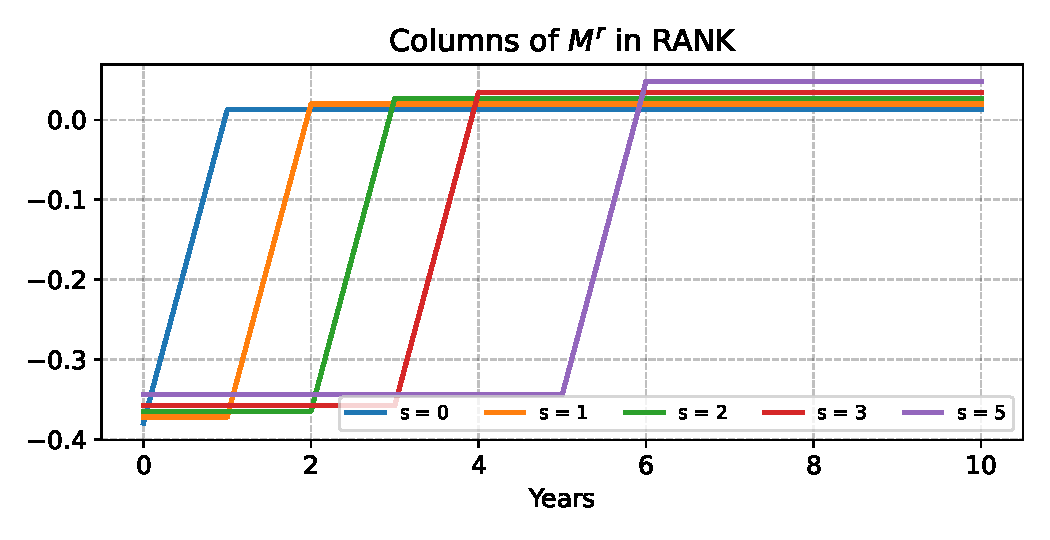
\includegraphics[width=0.5\linewidth]{figs/mon_Mr_RANK.pdf}
\end{figure}
\item <+->A rate cut at $s$: consumption is high up to $s$ and low after. It is almost a pure tilt
\end{itemize}
\end{frame}
%
\begin{frame}{Direct and indirect effects in RANK}
\begin{itemize}
\item <+->Annual model, as in the fiscal lectures: rate cut of 25 bp with persistence 0.4, $\sigma=2$, $B=0.25$\\
\begin{figure}[H]
\centering
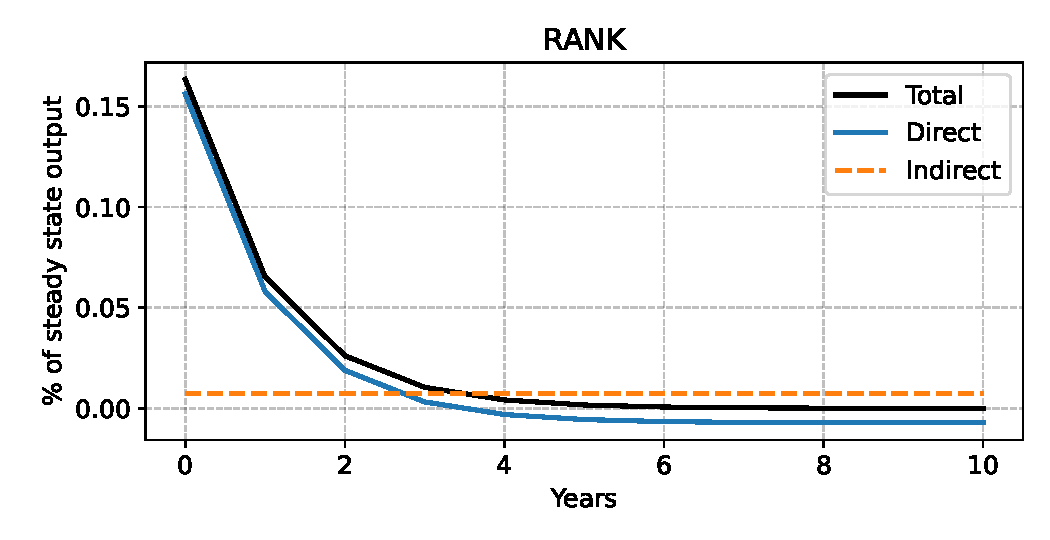
\includegraphics[width=0.55\linewidth]{figs/mon_decomp_RANK.pdf}
\end{figure}
\item <+->\textbf{96\% of the impact response is direct}
\item <+->Why: the MPC is $1-\beta\approx r$, about 0.02 a year, so income barely matters
\item <+-> Cochrane: the IS curve "ought to be renamed the 'intertemporal substitution' curve"
\end{itemize}
\end{frame}

\section{HANK}

\begin{frame}{Household problem in HANK}
\begin{itemize}
\item <+->Same household block as lecture 10:
\begin{align*}
v_{t}(z_{t},a_{t-1}) & =\max_{c_{t}}\frac{c_{t}^{1-\sigma}}{1-\sigma}+\beta\mathbb{E}_{t}\left[v_{t+1}(z_{t+1},a_{t})\right]\\
\text{s.t. }a_{t}+c_{t} & =(1+r_{t-1})a_{t-1}+Z_{t}z_{t}\\
\log z_{t+1} & =\rho_{z}\log z_{t}+\psi_{t+1},\quad\mathbb{E}[z_{t}]=1\\
a_{t} & \geq0
\end{align*}
\item <+->Everybody works the same, so income moves in proportion, $Z_{t}z_{t}$
\item <+->\textbf{Aggregate consumption:} $C_{t}^{hh}=\int c_{t}d\mathcal{D}_{t}$
\item <+->\textbf{Consumption function:} same object, $\boldsymbol{C}^{hh}=C^{hh}(\boldsymbol{Z},\boldsymbol{r})$
\item <+->No closed form: $\boldsymbol{M}$ and $\boldsymbol{M}^{r}$ are the household Jacobians with respect to $Z$ and $r$
\end{itemize}
\end{frame}
%
\begin{frame}{The Jacobian $\boldsymbol{M}^{r}$ in HANK}
\begin{itemize}
\item <+->Same $B>0$, same goods market, new household block\\
\begin{figure}[H]
\centering
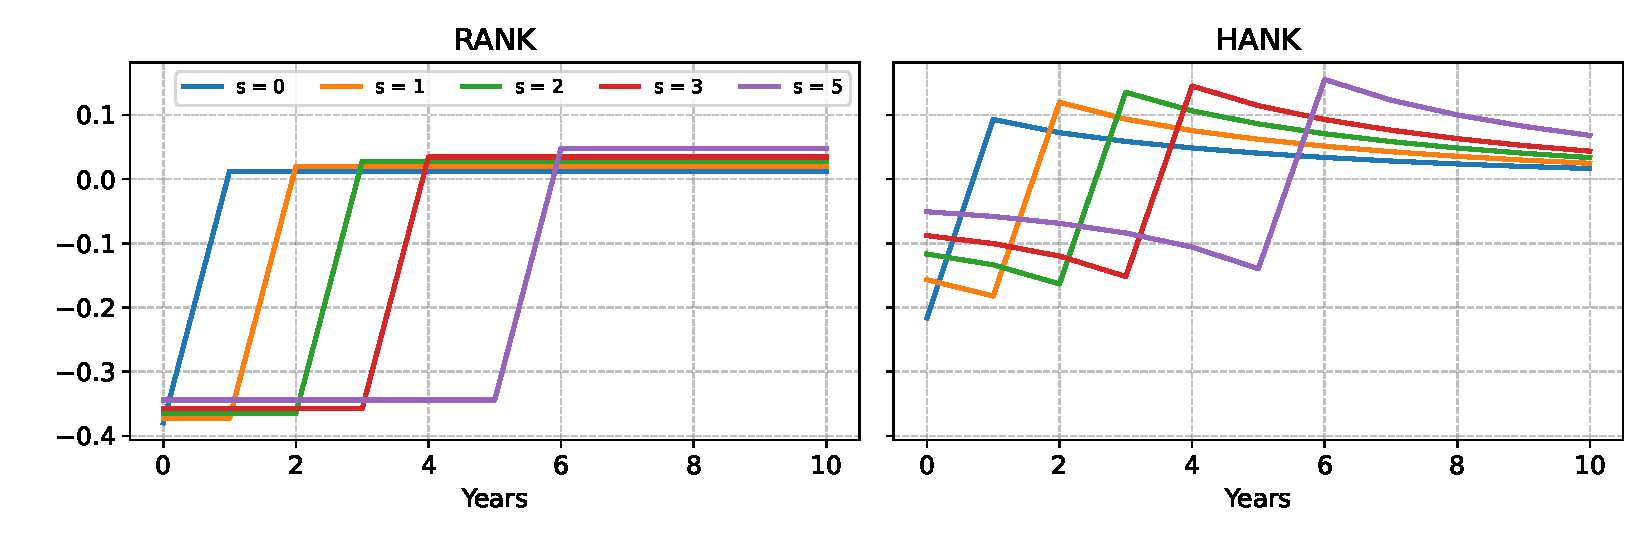
\includegraphics[width=0.85\linewidth]{figs/mon_Mr_compare.pdf}
\end{figure}
\item <+->\textbf{Households react less to $r$.} Why?
\begin{itemize}
\item Constrained households do not move: their Euler equation does not bind
\item Households close to the constraint move little: a buffer is worth keeping
\item A rate cut lowers interest income, which partly offsets substitution for savers
\end{itemize}
\end{itemize}
\end{frame}
%
\begin{frame}{$\boldsymbol{M}$ against $\boldsymbol{M}^{r}$}
\begin{itemize}
\item <+->Households react \textbf{more} to $Z$: high MPCs, as in lecture 10\\
\begin{figure}[H]
\centering
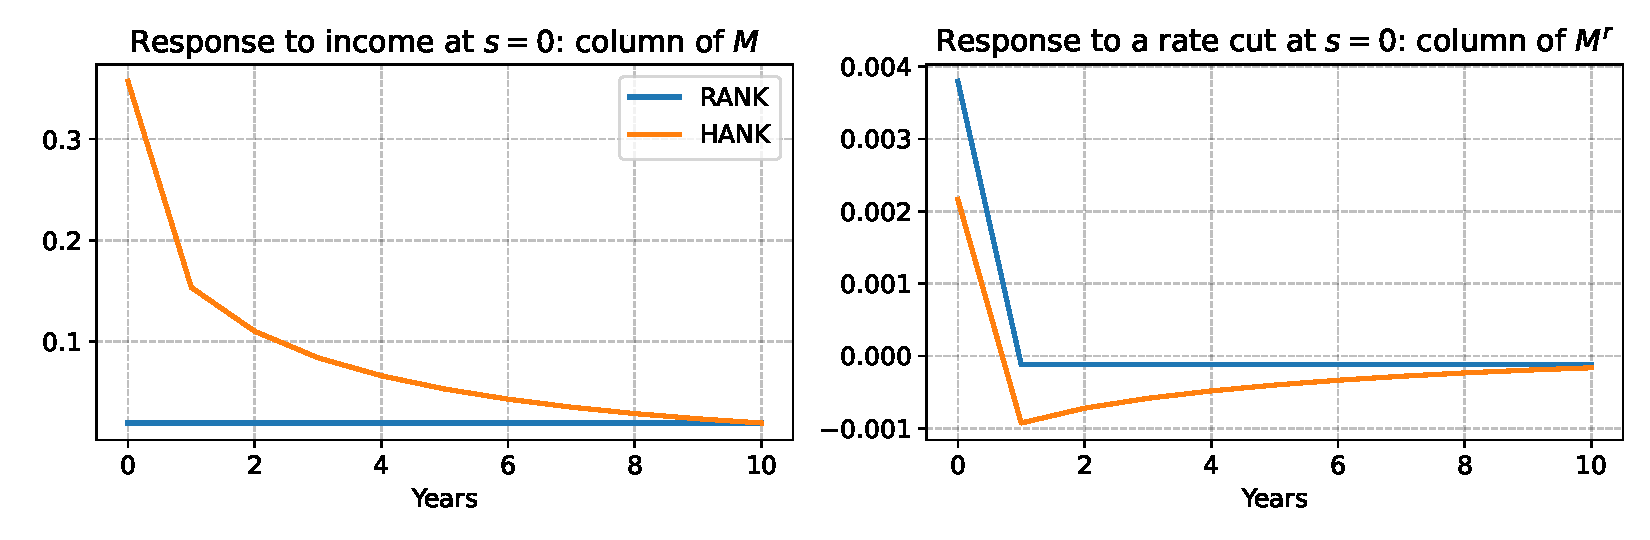
\includegraphics[width=0.85\linewidth]{figs/mon_M_vs_Mr.pdf}
\end{figure}
\item <+->First entry of $\boldsymbol{M}$: 0.02 in RANK, 0.36 in HANK
\item <+->The two Jacobians move in opposite directions
\item <+->Column of $\boldsymbol{M}^{r}$ is smaller in HANK and also decays: the cut is spent early and repaid slowly
\end{itemize}
\end{frame}
%
\begin{frame}{Direct and indirect effects in HANK}
\begin{itemize}
\item <+->Same shock, $B$ held fixed\\
\begin{figure}[H]
\centering
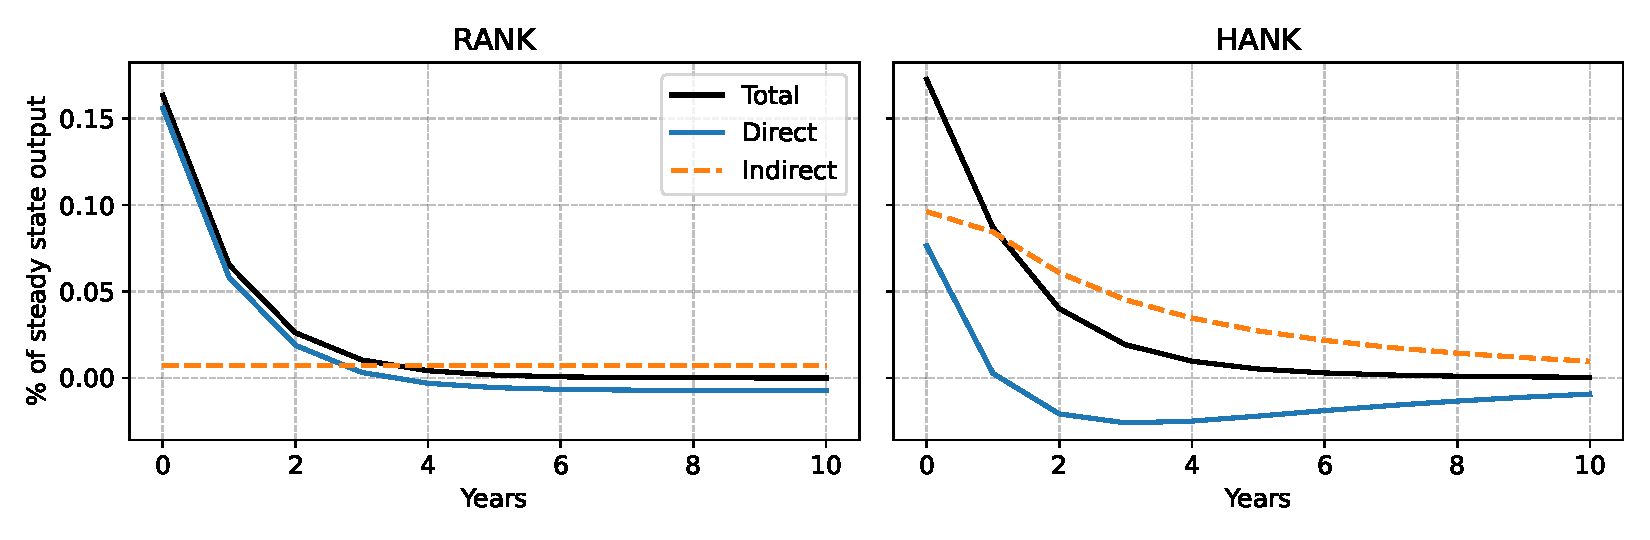
\includegraphics[width=0.85\linewidth]{figs/mon_decomp_compare.pdf}
\end{figure}
\item <+->Direct share of the impact response: \textbf{96\% in RANK, 44\% in HANK}
\item <+->Falls with liquidity: 25\% at $B=0.05$, 10\% at $B=0.01$
\item <+->Direct effect is negative after a couple of years: only the income effect keeps $C$ up
\end{itemize}
\end{frame}
%
\begin{frame}{What happens to the aggregate?}
\begin{itemize}
\item <+->Mechanism is completely different. What about the total?\\
\begin{figure}[H]
\centering
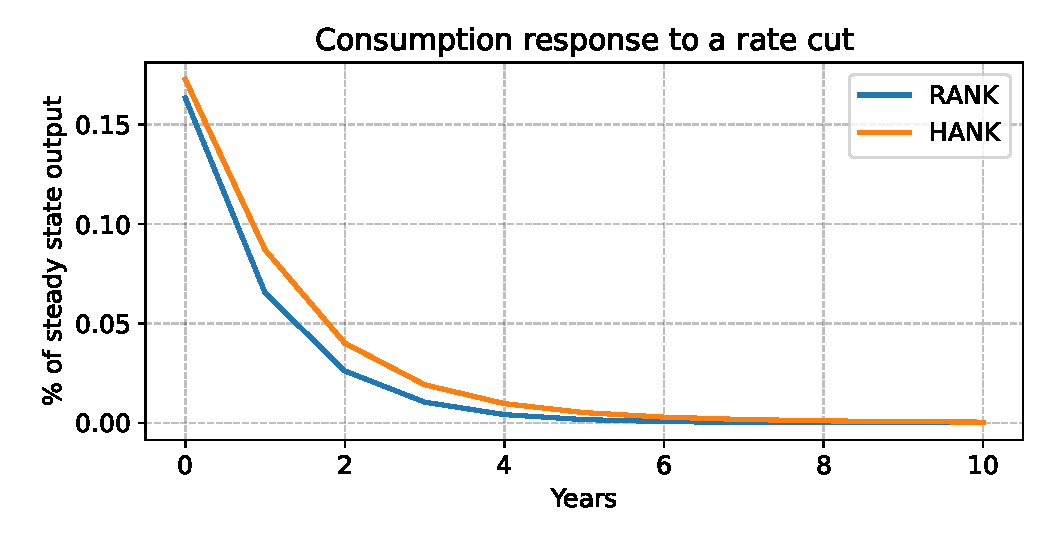
\includegraphics[width=0.55\linewidth]{figs/mon_total_compare.pdf}
\end{figure}
\item <+->Very similar!
\item <+->But a much smaller direct effect times a much larger multiplier
\end{itemize}
\end{frame}
%
\begin{frame}{Kaplan, Moll and Violante (2018): setup}
\begin{itemize}
\item <+->\textbf{Monetary Policy According to HANK}: the paper that named HANK, and the first to split monetary transmission into direct and indirect effects
\item <+->\textbf{Households:} two assets, as in Kaplan and Violante (2014)
\begin{itemize}
\item \textbf{Liquid} bonds $b$, return $r^{b}$, set by monetary policy
\item \textbf{Illiquid} assets $a$ (housing, equity), higher return $r^{a}$, but a cost $\chi(d,a)$ to deposit or withdraw
\item About a third are hand-to-mouth, many of them \textbf{wealthy}: high MPCs despite large illiquid wealth
\end{itemize}
\item <+->\textbf{Rest of the model:} NK firms with capital, a Taylor rule, and a government that adjusts lump-sum transfers $T$ to balance its budget
\item <+->\textbf{Experiment:} a cut in the Taylor rule. Decompose $C$ into the effect of each price path, holding the others fixed: $r^{b}$ (direct), and $w$, $T$, $r^{a}$ (indirect)
\end{itemize}
\end{frame}
%
\begin{frame}{Kaplan, Moll and Violante (2018): direct and indirect effects}
\begin{itemize}
\item <+->Monetary shock in HANK, quarterly\\
\begin{figure}[H]
\centering
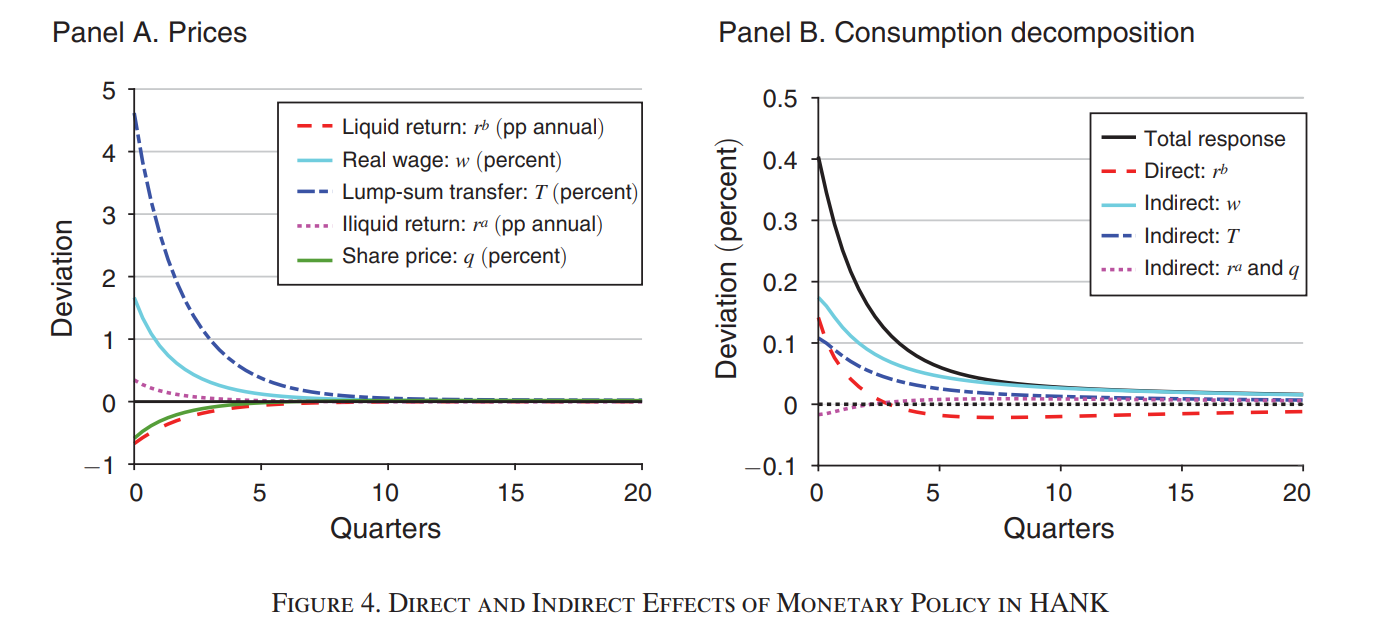
\includegraphics[width=0.7\linewidth]{figs/KMVFigure4.png}
\end{figure}
\item <+->\textbf{Direct effect: only 19\%} of the consumption response. Indirect: wages 51\%, transfers 32\%, illiquid return and share price $-2\%$
\item <+->\textbf{Why the direct effect is small:} hand-to-mouth households do not substitute over time, and savers lose interest income
\item <+->\textbf{Why the indirect effect is large:} higher labor income and transfers go to households with high MPCs
\end{itemize}
\end{frame}
%

\section{Equivalence}

\begin{frame}{Equivalence between RANK and HANK}
\begin{itemize}
\item <+->Similar aggregate response in HANK and RANK: \textbf{is this a coincidence?}
\item <+->\textbf{Werning (2015):} under some conditions, the output response to $r$ coincides in RANK and HANK
\begin{itemize}
\item zero liquidity, $B=0$, or
\item log utility, with income and borrowing limits proportional to aggregate income
\end{itemize}
\item <+->\textbf{In practice}, quantitatively the result is quite robust and hard to break
\end{itemize}
\end{frame}
%
\begin{frame}{Intuitive derivation: $B=0$}
\begin{itemize}
\item <+->No outside asset and $a_{t}\geq0$: nobody can save, so $c_{it}=Z_{t}z_{it}$ and $C_{t}=Z_{t}$
\item <+->The household with the strongest saving motive is on its Euler equation:
\[
\left(Z_{t}z\right)^{-\sigma}=\beta\left(1+r_{t}\right)Z_{t+1}^{-\sigma}\mathbb{E}\left[z'^{-\sigma}\mid z\right]
\]
\item <+->Income is proportional to aggregate income, so $z$ does not depend on $Z_{t}$. Then
\[
C_{t}^{-\sigma}=\tilde{\beta}\left(1+r_{t}\right)C_{t+1}^{-\sigma},\quad\tilde{\beta}=\beta\max_{z}\mathbb{E}\left[\left(z'/z\right)^{-\sigma}\mid z\right]
\]
\item <+->\textbf{The RANK Euler equation}, for any $\sigma$. Risk changes $\tilde{\beta}$, not the sensitivity to $r$
\item <+->Direct effect is zero, all of it is indirect: the opposite mechanism, the same aggregate
\end{itemize}
\end{frame}
%

\section{Full model}

\begin{frame}{Full model}
\begin{itemize}
\item <+->So far: real rate rule, real bonds, $\mu=1$, and everybody's income moves in proportion
\item <+->Drop these assumptions one at a time, starting each time from the monetary IKC:
\begin{enumerate}
\item \textbf{Markups:} $\mu>1$, so $p>0$ and a rate cut gives capital gains
\item \textbf{Nominal bonds:} surprise inflation revalues debt at $t=0$
\item \textbf{Unequal incidence:} the income share of each household moves with the cycle
\end{enumerate}
\item <+->Then we put all of them together
\item <+->We keep the real rate rule throughout: the shock is still $d\boldsymbol{r}$
\end{itemize}
\end{frame}
%
\begin{frame}{1. Markups: capital gains}
\vspace{-1mm}
\begin{itemize}
\item <+->With $\mu>1$, as in the fiscal lectures: $Z_{t}=\frac{1}{\mu}\left(Y_{t}-T_{t}\right)$, $d_{t}=\left(1-\frac{1}{\mu}\right)\left(Y_{t}-T_{t}\right)$, $A_{t}=p_{t}+B_{t}$
\item <+->The stock price is the present value of dividends, now discounted at the moving rate:
\[
p_{0}+d_{0}=d_{0}+\frac{d_{1}}{1+r_{0}}+\frac{d_{2}}{(1+r_{0})(1+r_{1})}+\dots
\]
\item <+->Differentiate. Dividends give the fiscal term, and a lower $r_{s}$ raises the value of all dividends after $s$, worth $p$:
\[
\text{cap}_{0}=dp_{0}+dd_{0}=\left(1-\frac{1}{\mu}\right)\boldsymbol{q}^{\prime}\left(d\boldsymbol{Y}-d\boldsymbol{T}\right)-\frac{p}{1+r_{ss}}\boldsymbol{q}^{\prime}d\boldsymbol{r}
\]
\item <+->A rate cut raises $p_{0}$: stockholders gain at $t=0$
\item <+->A stock is a long asset: the gain at $t=0$ offsets the lower returns later. Only the maturing part of wealth, $B$, is exposed to the rate
\end{itemize}
\end{frame}
%
\begin{frame}{1. Markups: IKC}
\begin{itemize}
\item <+->Consumption reacts to labor income, to the rate and to the capital gain:
\[
d\boldsymbol{Y}=\frac{1}{\mu}\boldsymbol{M}\left(d\boldsymbol{Y}-d\boldsymbol{T}\right)+\boldsymbol{M}^{r}d\boldsymbol{r}+\boldsymbol{m}\text{cap}_{0}
\]
\item <+->Replace $\text{cap}_{0}$:
\[
d\boldsymbol{Y}=\bar{\boldsymbol{M}}\left(d\boldsymbol{Y}-d\boldsymbol{T}\right)+\bar{\boldsymbol{M}}^{r}d\boldsymbol{r},\quad\bar{\boldsymbol{M}}^{r}\equiv\boldsymbol{M}^{r}-\frac{p}{1+r_{ss}}\boldsymbol{m}\boldsymbol{q}^{\prime}
\]
with $\bar{\boldsymbol{M}}=\frac{1}{\mu}\boldsymbol{M}+\left(1-\frac{1}{\mu}\right)\boldsymbol{m}\boldsymbol{q}^{\prime}$ as in the fiscal lectures
\item <+->\textbf{Same IKC}, with two new Jacobians
\item <+->$\boldsymbol{m}$ is small: stocks are held by wealthy households with low MPCs. The capital gain adds little demand, and $\bar{\boldsymbol{M}}$ is below $\boldsymbol{M}$ on impact
\item <+->\textbf{RANK:} $\boldsymbol{m}\boldsymbol{q}^{\prime}=\boldsymbol{M}^{RA}$, the capital gain is one more income gain
\end{itemize}
\end{frame}
%
\begin{frame}{2. Nominal bonds}
\vspace{-1mm}
\begin{itemize}
\item <+->Back to $\mu=1$. Debt issued at $t=-1$ pays $i_{ss}$, so surprise inflation lowers its real return at $t=0$:
\[
dr_{0}^{b}\approx-(1+r_{ss})d\pi_{0}
\]
\item <+->\textbf{Bondholders lose} $B_{ss}dr_{0}^{b}$, and \textbf{taxpayers gain} the same amount:
\[
d\boldsymbol{T}=B_{ss}\left(\boldsymbol{L}d\boldsymbol{r}+d\boldsymbol{r}^{b}\right),\quad d\boldsymbol{r}^{b}=(dr_{0}^{b},0,0,\dots)^{\prime}
\]
\item <+->\textbf{IKC:}
\[
d\boldsymbol{Y}=\boldsymbol{M}\left(d\boldsymbol{Y}-B_{ss}\boldsymbol{L}d\boldsymbol{r}\right)+\boldsymbol{M}^{r}d\boldsymbol{r}+B_{ss}\left(\boldsymbol{m}dr_{0}^{b}-\boldsymbol{M}d\boldsymbol{r}^{b}\right)
\]
\item <+->A rate cut raises $Y$, the W-NKPC gives $d\pi_{0}>0$, and inflation moves wealth from savers ($\boldsymbol{m}$) to taxpayers ($\boldsymbol{M}d\boldsymbol{r}^{b}$, higher MPCs): demand rises
\item <+->\textbf{Inflation is no longer irrelevant for output:} we need the W-NKPC, and $\kappa$ matters again
\end{itemize}
\end{frame}
%
\begin{frame}{3. Unequal incidence}
\vspace{-1mm}
\begin{itemize}
\item <+->Back to $\mu=1$ and real bonds. The income share of household $i$ now depends on aggregate income $Z_{t}$:
\[
c_{it}+a_{it}=(1+r_{t-1})a_{i,t-1}+Z_{t}\frac{z_{it}^{1+\zeta\log\left(Z_{t}/Z_{ss}\right)}}{\mathbb{E}\left[z_{it}^{1+\zeta\log\left(Z_{t}/Z_{ss}\right)}\right]}
\]
\item <+->Aggregate income is still $Z_{t}$. Only its split moves
\begin{itemize}
\item $\zeta<0$: when $Z$ rises, income shifts towards low-$z$ households, and risk falls
\item $\zeta>0$: the opposite
\end{itemize}
\item <+->Households still only see $\boldsymbol{Z}$ and $\boldsymbol{r}$. So the IKC is unchanged, with new iMPCs $\tilde{\boldsymbol{M}}$:
\[
d\boldsymbol{Y}=\tilde{\boldsymbol{M}}\left(d\boldsymbol{Y}-d\boldsymbol{T}\right)+\boldsymbol{M}^{r}d\boldsymbol{r}
\]
\item <+->$\zeta<0$: extra income goes to high-MPC households and lowers precautionary saving, so $\tilde{\boldsymbol{M}}$ is above $\boldsymbol{M}$ on impact
\item <+->Still $\boldsymbol{q}^{\prime}\tilde{\boldsymbol{M}}=\boldsymbol{q}^{\prime}$. Cost: tax changes also move inequality
\end{itemize}
\end{frame}
%
\begin{frame}{All together}
\vspace{-1mm}
\begin{itemize}
\item <+->With $d\boldsymbol{G}=d\boldsymbol{B}=\boldsymbol{0}$:
\[
d\boldsymbol{Y}=\bar{\boldsymbol{M}}\left(d\boldsymbol{Y}-d\boldsymbol{T}\right)+\bar{\boldsymbol{M}}^{r}d\boldsymbol{r}+\boldsymbol{m}B_{ss}dr_{0}^{b}
\]
\[
d\boldsymbol{T}=B_{ss}\left(\boldsymbol{L}d\boldsymbol{r}+d\boldsymbol{r}^{b}\right),\quad dr_{0}^{b}\approx-(1+r_{ss})d\pi_{0}
\]
\item <+->Each feature is one term:
\begin{itemize}
\item \textbf{Markups:} $\bar{\boldsymbol{M}}$ and $\bar{\boldsymbol{M}}^{r}$, the capital gain on stocks
\item \textbf{Nominal bonds:} $B_{ss}\left(\boldsymbol{m}dr_{0}^{b}-\boldsymbol{M}d\boldsymbol{r}^{b}\right)$, savers' MPCs against taxpayers' MPCs
\item \textbf{Unequal incidence:} $\tilde{\boldsymbol{M}}$ in place of $\boldsymbol{M}$, also inside $\bar{\boldsymbol{M}}$
\end{itemize}
\item <+->In RANK none of this matters: one household gets all transfers, so $\boldsymbol{m}dr_{0}^{b}=\boldsymbol{M}d\boldsymbol{r}^{b}$ and $\bar{\boldsymbol{M}}=\tilde{\boldsymbol{M}}=\boldsymbol{M}$
\item <+->\textbf{Second session:} Auclert (2019) reads these terms as redistribution between winners and losers with different MPCs
\end{itemize}
\end{frame}
%

\section{Forward guidance}

\begin{frame}{The forward guidance puzzle in RANK}
\begin{itemize}
\item <+->From the iterated Euler equation:
\[
\log C_{t}=\log C_{ss}-\frac{1}{\sigma}\sum_{s\geq0}\log\left(\beta\left(1+r_{t+s}\right)\right)
\]
\item <+->A cut in 10 years moves consumption today as much as a cut now
\item <+->With inflation responding, the effect grows with the horizon\\
\begin{figure}[H]
\centering
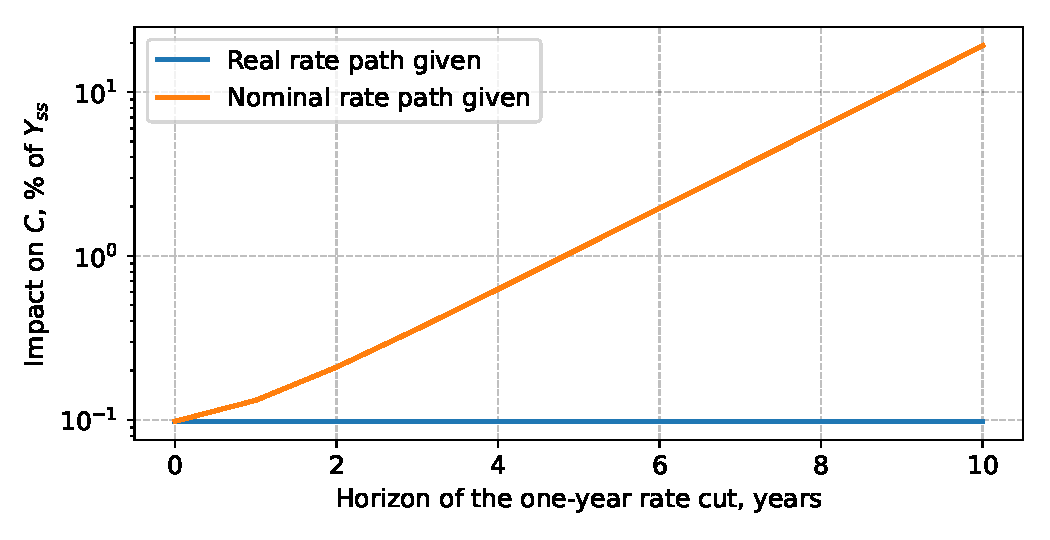
\includegraphics[width=0.5\linewidth]{figs/fg_RANK.pdf}
\end{figure}
\item <+->This is the \textbf{forward guidance puzzle} (Del Negro, Giannoni and Patterson, 2013)
\end{itemize}
\end{frame}
%
\begin{frame}{Does HANK solve it? Not under Werning}
\begin{itemize}
\item <+->Direct corollary of Werning (2015): same aggregate Euler equation, so the same sensitivity to current and \textbf{future} rates
\item <+->Forward guidance is exactly as powerful as in RANK: at $B=0$ for any $\sigma$, and at $B>0$ with log utility
\item <+->Away from the benchmark, Werning finds that consumption is likely to be \textbf{more} sensitive, especially to future rates
\begin{itemize}
\item Countercyclical risk: future income lowers uncertainty, precautionary saving falls
\item $\sigma>1$: lower rates raise the value of assets relative to income
\end{itemize}
\item <+->So incomplete markets alone do not solve the puzzle
\end{itemize}
\end{frame}

%
\begin{frame}{With cyclical income: McKay, Nakamura and Steinsson (2016)}
\begin{itemize}
\item <+->HANK with uninsurable risk and borrowing constraints, $B$ of 1.4 times annual GDP
\item <+->Experiment: real rate 50 bp lower for one quarter, 20 quarters ahead
\begin{itemize}
\item Complete markets: output up by 25 bp at once
\item Incomplete markets: about 10 bp, and essentially zero at 10 years
\end{itemize}
\item <+->\textbf{Why:} a precautionary saving effect tempers the response to future rates
\begin{itemize}
\item The chance of hitting the constraint before the rate falls rises with the horizon
\end{itemize}
\item <+->\textbf{Why not Werning?} In their words, Werning assumes that income, constraints and assets scale with aggregate income. In their model
\begin{itemize}
\item the extra income goes disproportionately to high earners
\item the shock raises incomes relative to assets
\end{itemize}
\item <+->Taxes are paid only by the highest productivity type
\end{itemize}
\end{frame}
%
\begin{frame}{Forward guidance in our model}
\begin{itemize}
\item <+->Impact of a one-year rate cut at horizon $s$, relative to RANK, $\sigma=2$\\
\begin{figure}[H]
\centering
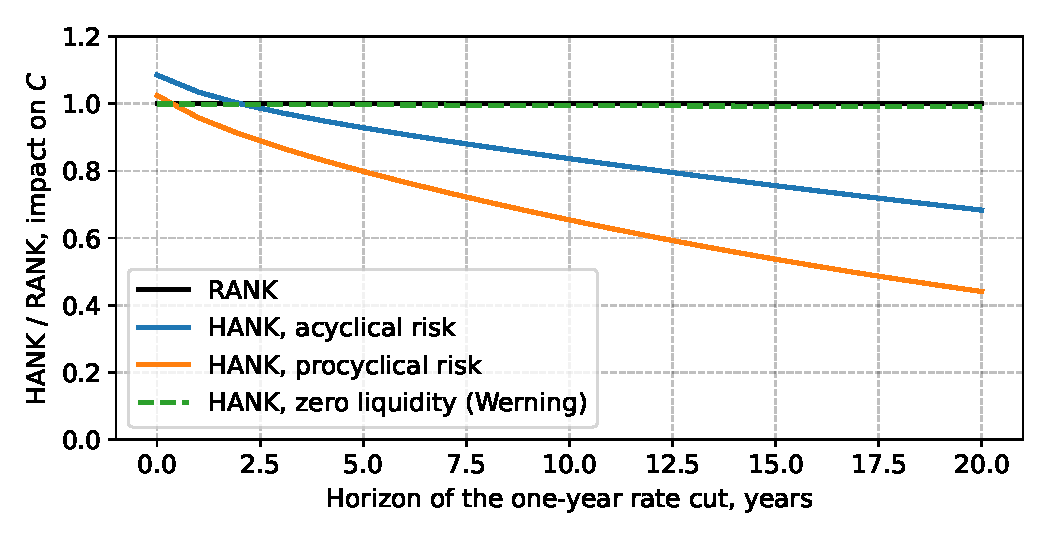
\includegraphics[width=0.55\linewidth]{figs/fg_HANK.pdf}
\end{figure}
\item <+->\textbf{Zero liquidity} (Werning), $B=10^{-5}$: as strong as in RANK at all horizons
\item <+->\textbf{Acyclical risk}, $B=0.25$: 0.84 of RANK at 10 years. A boom raises income but not liquidity, so households save a bit more today
\item <+->\textbf{Procyclical risk}, $\zeta=0.3$: 0.65 at 10 years, 0.44 at 20. The boom also raises risk
\item <+->Same message as McKay et al.: what matters is who gets the extra income
\end{itemize}
\end{frame}
%

\section{Recap}

%
\begin{frame}{Summary of the first session}
\begin{itemize}
\item <+->\textbf{RANK:} monetary policy is intertemporal substitution, almost all direct
\item <+->\textbf{HANK:} less direct, more indirect, close to the same aggregate
\begin{itemize}
    \item <+->\textbf{Fiscal policy:} HANK changes the multipliers. 
    \item <+->\textbf{Monetary policy:} less direct, more indirect, close to the same aggregate
\end{itemize}
\item <+->Equivalence holds when incidence, liquidity and risk do not move with the cycle
\item <+->\textbf{Forward guidance:} as strong as in RANK under Werning, weaker with procyclical income risk
\item <+->\textbf{Next time:} redistribution and the role of investment under sticky expectations
\end{itemize}
\end{frame}
%

\end{document}
